\subsection{Gram-Schmidt Orthogonalization Process}\label{subsec:Gram-Schmidt_Orthogonalization}
\begin{definition}[Span]\label{def:Span}
  The \emph{span} of a vector or set of vectors, is a linear combination of all possible vectors.
  For example, if $S = \lbrace u_{1}, u_{2} \rbrace$, then $\Span(S) = \lbrace c_{1}u_{1} + c_{2}u_{2} : c_{1}, c_{2} \in \RealNumbers \rbrace$.
\end{definition}

\begin{definition}[Projection]\label{def:Vector_Projection}
  The \emph{projection} of a vector onto another is the amount of one vector that is in the same direction as another.
  It is denoted $\Proj{u_{2}}{u_{1}}$, and is said ``the projection of $u_{2}$ on $u_{1}$''.
  It is defined as:
  \begin{equation}\label{eq:Vector_Projection}
    \Proj{u_{2}}{u_{1}} = \frac{u_{2} \cdot u_{1}}{u_{1} \cdot u_{1}} u_{1}
  \end{equation}
\end{definition}

\begin{definition}[Rejection]\label{def:Vector_Rejection}
  The \emph{rejection} of a vector from another vector is the amount that one vector is \textbf{not} in the same direction as another, in an orthogonal fashion.
  This can be seen graphically in \Cref{fig:Vector_Projection_Rejection}.
  It is denoted $\Rej{u_{2}}{u_{1}}$, and is said ``the rejection of $u_{2}$ from $u_{1}$''.
  If is defined as:
  \begin{equation}\label{eq:Vector_Rejection}
    \begin{aligned}
      \Rej{u_{2}}{u_{1}} &= u_{2} - \frac{u_{2} \cdot u_{1}}{u_{1} \cdot u_{1}} u_{1} \\
      \Rej{u_{2}}{u_{1}} &= u_{2} - \Proj{u_{2}}{u_{1}}
    \end{aligned}
  \end{equation}
\end{definition}

\begin{figure}[h!tbp]
  \centering
  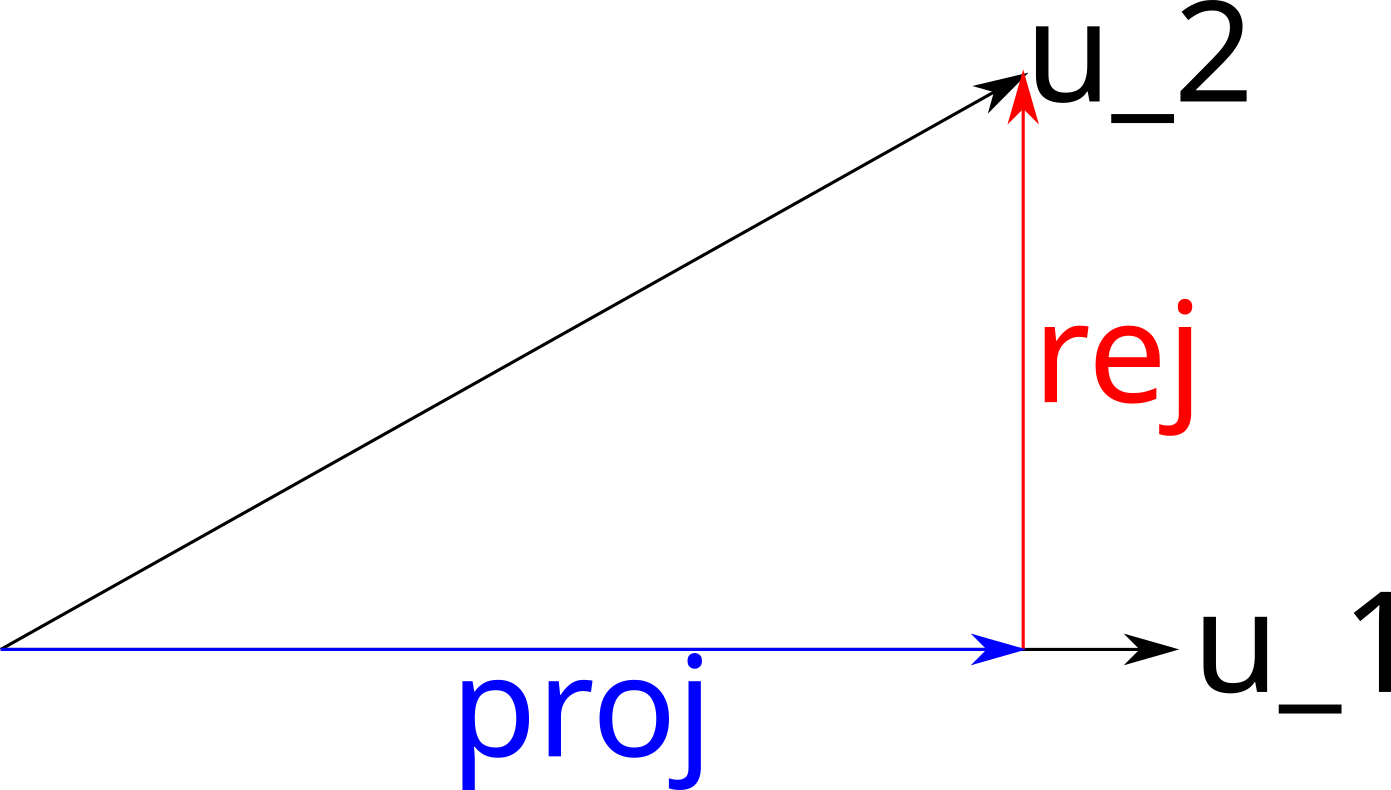
\includegraphics[scale=0.50]{./Vector_Projection_Rejection.png}
  \caption{Vector Projection and Rejection}
  \label{fig:Vector_Projection_Rejection}
\end{figure}

\begin{theorem}[Gram-Schmidt Orthogonalization Process]\label{thm:Gram-Schmidt_Orthogonalization}
  Given $m$ \nameref{def:Linearly_Independent} vectors in $\RealNumbers^{n}$ ($m$ vectors, each with $n$ components),
  \begin{equation*}
    S = \lbrace u_{1}, u_{2}, \ldots, u_{m} \rbrace, \: n \geq m
  \end{equation*}

  To find $V = \lbrace v_{1}, v_{2}, \ldots, v_{m} \rbrace$ orthogonal vectors where $\Span(V) = \Span(S)$.

  We can find such vectors by repeatedly using the \nameref{def:Vector_Rejection} of the original vector from the first orthogonal vector.
  So, the process boils down to:
  \begin{equation}\label{eq:Gram-Schmidt_Orthogonalization}
    \begin{aligned}
      v_{1} &= u_{1} \\
      v_{2} &= u_{2} - \Rej{u_{2}}{v_{1}} \\
      &= u_{2} - \frac{u_{2} \cdot v_{1}}{v_{1} \cdot v_{1}} v_{1} \\
      v_{3} &= u_{3} - \frac{u_{3} \cdot v_{1}}{v_{1} \cdot v_{1}} v_{1} - \frac{u_{3} \cdot v_{2}}{v_{2} \cdot v_{2}} v_{2} \\
      &\vdots \\
      v_{m} &= u_{m} - \frac{u_{m} \cdot v_{1}}{v_{1} \cdot v_{1}} v_{1} - \cdots - \frac{u_{m} \cdot v_{m-1}}{v_{m-1} \cdot v_{m-1}} v_{m-1}
    \end{aligned}
  \end{equation}
\end{theorem}

\begin{example}[Lecture 21, Example 1]{Find Orthogonal Vector}
  Given three vectors in $\RealNumbers^{4}$, find $\lbrace v_{1}, v_{2}, v_{3} \rbrace$ where each element is mutually orthogonal, and the \nameref{def:Span} $\Span(S)$ remains the same.
  \begin{equation*}
    S = \lbrace (1, 2, -1, 2), (2, 3, -1, 1), (0, 2, -1, 4) \rbrace
  \end{equation*}
  \tcblower{}
  From \nameref{thm:Gram-Schmidt_Orthogonalization} (\Cref{eq:Gram-Schmidt_Orthogonalization}), we already know how to solve this.
  \begin{align*}
    v_{1} &= u_{1} \\
          &= (1, 2, -1, 2)
  \end{align*}

  Now, we can solve for the second orthogonal vector.
  \begin{align*}
    v_{2} &= u_{2} - \frac{u_{2} \cdot v_{1}}{v_{1} \cdot v_{1}} v_{1} \\
          &= u_{2} - \frac{(2, 3, -1, 1) \cdot (1, 2, -1, 1)}{(1, 2, -1, 1) \cdot (1, 2, -1, 1)} v_{1} \\
          &= u_{2} - \frac{2 + 6 + 1 + 2}{1 + 4 + 1 + 4} v_{1} \\
          &= (2, 3, -1, 1) - \frac{11}{10} (1, 2, -1, 2) \\
          &= \frac{(20, 30, -10, 10) - 11 (1, 2, -1, 2)}{10} \\
    v_{2} &= (\frac{9}{10}, \frac{8}{10}, \frac{1}{10}, \frac{-12}{10}) \\
    \intertext{The scaling is unimportant here, so we can actually drop the fractional part.}
    v_{2} &= (9, 8, 1, -12)
  \end{align*}

  Lastly, we solve for the last orthogonal vector.
  \begin{align*}
    v_{3} &= u_{3} - \frac{u_{3} \cdot v_{1}}{v_{1} \cdot v_{1}} v_{1} - \frac{u_{3} \cdot v_{2}}{v_{2} \cdot v_{2}} \\
          &= u_{3} - \frac{(0, 2, -1, 4) \cdot (1, 2, -1, 2)}{10} v_{1} - \frac{(0, 2, -1, 4) \cdot (9, 8, 1, -12)}{(9,8,1,-12) \cdot (9,8,1,-12)} v_{2} \\
          &= u_{3} - \frac{0+4+1+8}{10} v_{1} - \frac{-33}{290} v_{2} \\
          &= (0, 2, -1, 4) - \frac{13}{10}(1,2,-1,2) + \frac{33}{290} (9, 8, 1, -12) \\
    v_{3} &= (\frac{-8}{29}, \frac{9}{29}, \frac{12}{29}, \frac{1}{29}) \\
    \intertext{The scaling is unimportant.}
    v_{3} &= (-8, 9, 12, 1)
  \end{align*}
\end{example}

\begin{example}[Lecture 21, Example 2]{Gram-Schmidt on Matrices}
  Given the \nameref{def:Real_Symmetric_Matrix} $A$, determine an \nameref{def:Orthogonal_Matrix} that implements a \nameref{def:Diagonalization}.
  \begin{equation*}
    A =
    \begin{pmatrix}
      3 & 2 & 4 \\
      2 & 0 & 2 \\
      4 & 2 & 3
    \end{pmatrix}
  \end{equation*}
  \tcblower{}
  Start by finding the \nameref{def:Eigenvalue}s, and then the \nameref{def:Eigenvector}s.
  \begin{align*}
    A - \lambda I &=
                    \begin{pmatrix}
                      3 - \lambda & 2 & 4 \\
                      2 & 0 - \lambda & 2 \\
                      4 & 2 & 3 - \lambda
                    \end{pmatrix} \\
    \intertext{We can make finding the \nameref{def:Determinant} easier by performing some \nameref{def:Elementary_Column_Op}s.
    Refer back to \Cref{subsubsec:Create_0s_Determinants} for how these affect the determinant's outcome.}
    &\grstep{-2c_{2} + c_{3}}
      \begin{pmatrix}
        3 - \lambda & 2 & 0 \\
        2 & - \lambda & 2 + 2 \lambda \\
        4 & 2 & -1 - \lambda
      \end{pmatrix} \\
    \det(A - \lambda I) &= (1 + \lambda) \det
                          \begin{pmatrix}
                            3 - \lambda & 2 & 0 \\
                            2 & -\lambda & 2 \\
                            4 & 2 & -1
                          \end{pmatrix} \\
    \intertext{Finding the \nameref{def:Determinant} by expanding the first row.}
                  &= (1 + \lambda) \bigl( (3-\lambda) (\lambda - 4) - 2(-2 - 8) \bigr) \\
                  &= (1 + \lambda) (3\lambda - \lambda^{2} + 4 \lambda - 12 + 20) \\
                  &= (1 + \lambda) (-\lambda^{2} + 7\lambda + 8) \\
                  &= (1 + \lambda) (\lambda + 1) (-\lambda + 8)
  \end{align*}
  We get \nameref{def:Eigenvalue}s if and only if $\det(A - \lambda I) = 0$.
  So, we have two \textbf{distinct} eigenvalues:
  \begin{description}[noitemsep]
  \item[$\lambda = -1$] With algebraic multiplicity 2.
  \item[$\lambda = 8$] With algebraic multiplicity 1.
  \end{description}

  Now, finding the \nameref{def:Eigenvector}s. \\
  For $\lambda = -1$:
  \begin{align*}
    \begin{pmatrix}
      4 & 2 & 4 \\
      2 & 1 & 2 \\
      4 & 2 & 4
    \end{pmatrix}
              \begin{pmatrix}
      x_{1} \\ x_{2} \\ x_{3}
    \end{pmatrix} &=
                    \begin{pmatrix}
                      0 \\ 0 \\ 0
                    \end{pmatrix} \\
    \grstep{\substack{-2r_{2} + r_{1} \\ -2r_{2} + r_{3}}}
    \begin{pmatrix}
      0 & 0 & 0 \\
      2 & 1 & 2 \\
      0 & 0 & 0
    \end{pmatrix}
              \begin{pmatrix}
                x_{1} \\ x_{2} \\ x_{3}
              \end{pmatrix} &=
                              \begin{pmatrix}
                                0 \\ 0 \\ 0
                              \end{pmatrix} \\
    \intertext{Convert to system of linear equations.}
    2x_{1} + x_{2} + 2x_{3} &= 0 \\
    \intertext{Solve the system.}
    x_{1} &= \frac{-1}{2} x_{2} - x_{3} \\
    x_{2} &= x_{2} \\
    x_{3} &= x_{3}
  \end{align*}

  So, the \nameref{def:Eigenvector} for $\lambda = -1$ is:
  \begin{align*}
    \begin{pmatrix}
      x_{1} \\ x_{2} \\ x_{3}
    \end{pmatrix} &=
                    \begin{pmatrix}
                      \frac{-1}{2} x_{2} - x_{3} \\ x_{2} \\ x_{3}
                    \end{pmatrix} \\
    &= x_{2}
      \begin{pmatrix}
        \frac{-1}{2} \\ 1 \\ 0
      \end{pmatrix} + x_{3}
    \begin{pmatrix}
      -1 \\ 0 \\ 1
    \end{pmatrix} \\
    \intertext{Where $x_{2} \neq 0$ and $x_{3} \neq 0$ simultaneously.}
  \end{align*}

  For $\lambda = -1$, we have two \nameref{def:Eigenvector}s, but they are not distinct.

  For $\lambda = 8$:
  \begin{align*}
    \begin{pmatrix}
      -5 & 2 & 4 \\
      2 & -8 & 2 \\
      4 & 2 & -5
    \end{pmatrix}
              \begin{pmatrix}
      x_{1} \\ x_{2} \\ x_{3}
    \end{pmatrix} &=
                    \begin{pmatrix}
                      0 \\ 0 \\ 0
                    \end{pmatrix} \\
    \grstep{r_{3} + r_{1}}
    \begin{pmatrix}
      -1 & 4 & -1 \\
      2 & -8 & 2 \\
      4 & 2 & -5
    \end{pmatrix}
              \begin{pmatrix}
                x_{1} \\ x_{2} \\ x_{3}
              \end{pmatrix} &=
                              \begin{pmatrix}
                                0 \\ 0 \\ 0
                              \end{pmatrix} \\
    \grstep{\substack{2r_{1} + r_{2} \\ 4r_{1} + r_{3}}}
    \begin{pmatrix}
      -1 & 4 & -1 \\
      0 & 0 & 0 \\
      0 & 18 & -9
    \end{pmatrix}
              \begin{pmatrix}
                x_{1} \\ x_{2} \\ x_{3}
              \end{pmatrix} &=
                              \begin{pmatrix}
                                0 \\ 0 \\ 0
                              \end{pmatrix} \\
    \intertext{Convert to system of linear equations.}
    -x_{1} + 4x_{2} - x_{3} &= 0 \\
    18x_{2} - 9x_{3} &= 0 \\
    \intertext{Solve the system.}
    x_{3} &= 2x_{2} \\
    x_{1} &= 2x_{2} \\
    x_{2} &= x_{2}
  \end{align*}

  So, the \nameref{def:Eigenvector} for $\lambda = 8$ is:
  \begin{align*}
    \begin{pmatrix}
      x_{1} \\ x_{2} \\ x_{3}
    \end{pmatrix} &=
                    \begin{pmatrix}
                      2x_{2} \\ x_{2} \\ 2x_{2}
                    \end{pmatrix} \\
    &= x_{2}
      \begin{pmatrix}
        2 \\ 1 \\ 2
      \end{pmatrix}
    \intertext{Where $x_{2} \neq 0$}
  \end{align*}

  From the gathered \nameref{def:Eigenvector}s, set our vectors to be:
  \begin{align*}
    u_{1} &= (-1, 2, 0) \\
    u_{2} &= (-1, 0, 1) \\
    u_{3} &= (2, 1, 2) \\
    \intertext{Checking if the vectors' orthogonality.}
    u_{1} \cdot u_{2} &= \left( \frac{-1}{2} \right) (-1) + 1 (0) + 0 (1) \\
          &= \frac{1}{2} \\
          &\neq 0 \\
    u_{1} \cdot u_{3} &= 0 \\
    u_{2} \cdot u_{3} &= 0
  \end{align*}

  We can now use \nameref{thm:Gram-Schmidt_Orthogonalization} to find a new set of vectors which \textit{are} orthogonal.
  \begin{align*}
    v_{1} &= u_{1} \\
    v_{1} &= (-1, 2, 0)
  \end{align*}

  Next,
  \begin{align*}
    v_{2} &= u_{2} - \frac{u_{2} \cdot v_{1}}{v_{1} \cdot v_{1}} v_{1} \\
          &= (-1, 0, 1) - \frac{1}{5} (-1, 2, 0) \\
          &= (\frac{-4}{5}, \frac{-2}{5}, 1) \\
          &= (4, 2, -5) \\
  \end{align*}

  Lastly,
  \begin{align*}
    v_{3} &= u_{3} - \frac{u_{3} \cdot v_{1}}{v_{1} \cdot v_{1}} v_{1} - \frac{u_{3} \cdot v_{2}}{v_{2} \cdot v_{2}} v_{2} v_{2} \\
    \intertext{Remember, $u_{3}$ was already orthogonal to $u_{1}$ and $u_{2}$, so it is orthogonal to $v_{1}$ and $v_{2}$ already.}
          &= u_{3} \\
    v_{3} &= (2, 1, 2)
  \end{align*}

  Lastly, we need to normalize each column, to make an \nameref{def:Orthogonal_Matrix}.
  \begin{align*}
    \Magnitude{v_{1}} &= \sqrt{5} \\
    \Magnitude{v_{2}} &= \sqrt{45} \\
    \Magnitude{v_{3}} &= 3
  \end{align*}

  Thus, our \nameref{def:Orthogonal_Matrix}, $Q$ implements a \nameref{def:Diagonalization} of $A$ whose product is $D$.
  \begin{align*}
    Q &=
        \begin{pmatrix}
          \frac{-1}{\sqrt{5}} & \frac{4}{\sqrt{45}} & \frac{2}{3} \\
          \frac{2}{\sqrt{5}} & \frac{2}{\sqrt{45}} & \frac{1}{3} \\
          0 & \frac{-5}{\sqrt{45}} & \frac{2}{3}
        \end{pmatrix} \\
    D &=
        \begin{pmatrix}
          -1 & 0 & 0 \\
          0 & -1 & 0 \\
          0 & 0 & 8
        \end{pmatrix}
  \end{align*}
\end{example}

\subsubsection{Determine if Vector is in Span}\label{subsubsec:Determine_Vector_In_Span}
Similar to how we determine a new set of orthogonal vectors using the \nameref{thm:Gram-Schmidt_Orthogonalization}, we can use the \nameref{def:Vector_Rejection} to determine if another vector is \textbf{in} the space created by the \nameref{def:Span} $\Span(S)$.

In short, if a vector is inside of a space, then its \nameref{def:Vector_Rejection} from the space is zero.
\begin{equation*}
  \Rej{w}{S} = 0
\end{equation*}

Thus, to verify that a vector $w$ \textbf{is} inside a \nameref{def:Span} $S$ created by a set of vectors, you must verify \Cref{eq:Verify_Vector_In_Span}.
\begin{equation}\label{eq:Verify_Vector_In_Span}
  w = \Proj{w}{S}
\end{equation}

That means that the \nameref{def:Vector_Projection} onto the span is defined as a linear combination of the orthogonal vectors that create the space.
\begin{equation*}
  \Proj{w}{S} = c_{1} v_{1} + c_{2} v_{2} + \cdots + c_{m} v_{m}
\end{equation*}

From our earlier discussion (and visualized in \Cref{fig:Vector_Projection_Rejection}), we know:
\begin{equation*}
  w - \Proj{w}{S} = \Rej{w}{S}
\end{equation*}

Using all this information, we can find an equation defining $\Proj{w}{S}$.
\begin{align*}
  w - \Proj{w}{S} &= \Rej{w}{S} \\
  w - c_{1} v_{1} - c_{2} v_{2} - \cdots - c_{m} v_{m} &= \Rej{w}{S} \\
  \intertext{We can solve for $v_{1}$ by using dot products. This works because the \nameref{def:Vector_Rejection} \textit{must} be orthogonal to all vectors that construct the \nameref{def:Span}.}
  (w - c_{1} v_{1} - c_{2} v_{2} - \cdots - c_{m} v_{m}) \cdot v_{1} &= \Rej{w}{S} \cdot v_{1} \\
  (w \cdot v_{1}) - c_{1} (v_{1} \cdot v_{1}) - c_{2} (v_{2} \cdot v_{1}) - \cdots - c_{m} (v_{m} \cdot v_{1}) &= 0 \\
  \intertext{Because each of the \nameref{def:Span}-constructing vectors are orthogonal to each other, their dot products is zero.}
  (w \cdot v_{1}) - c_{1} (v_{1} \cdot v_{1}) - c_{2} (0) - \cdots - c_{m} (0) &= 0 \\
  w \cdot v_{1} &= c_{1} (v_{1} \cdot v_{1}) \\
  c_{1} &= \frac{w \cdot v_{1}}{v_{1} \cdot v_{1}} \\
  \intertext{You can solve for the other coefficients the exact same way, yielding similar-looking equations.}
  \Proj{w}{S} &= \frac{w \cdot v_{1}}{v_{1} \cdot v_{1}} v_{1} + \frac{w \cdot v_{2}}{v_{2} \cdot v_{2}} v_{2} + \cdots + \frac{w \cdot v_{m}}{v_{m} \cdot v_{m}} v_{m}
\end{align*}

This shows the general equation to find the \nameref{def:Vector_Projection} of $w$ onto a \nameref{def:Span} $S$.
\begin{equation}\label{eq:Vector_Projected_onto_Span}
  \Proj{w}{S} = \frac{w \cdot v_{1}}{v_{1} \cdot v_{1}} v_{1} + \frac{w \cdot v_{2}}{v_{2} \cdot v_{2}} v_{2} + \cdots + \frac{w \cdot v_{m}}{v_{m} \cdot v_{m}} v_{m}
\end{equation}

\begin{blackbox}
  Because \Cref{eq:Vector_Projected_onto_Span} yields another vector, we can find the distance from the end of $w$ to the \nameref{def:Span} $S$ by using the magnitude of the \nameref{def:Vector_Rejection} of $w$ from $S$.
\end{blackbox}

%%% Local Variables:
%%% mode: latex
%%% TeX-master: "../../Math_333-MatrixAlg_ComplexVars-Reference_Sheet"
%%% End:
